\documentclass[a4paper,10pt]{report}

\usepackage{tikz}
\usetikzlibrary{shadows.blur}
\usetikzlibrary{shapes.symbols}

\usepackage{fancybox, graphicx}
\usepackage{hyperref}
\usepackage{amsmath}
\usepackage{amssymb}
\usepackage{xspace}
\pagestyle{headings}
%\usepackage[margin=1.2in]{geometry}
\usepackage[left=2cm, right=2cm, top=2.5cm, bottom=2cm]{geometry}
\usepackage{float}
\restylefloat{table}
\usepackage{listings}
\usepackage{color}
\definecolor{gray}{rgb}{0.4,0.4,0.4}
\definecolor{darkblue}{rgb}{0.0,0.0,0.58}
\definecolor{attributeColor}{rgb}{0.96,0.517,0.29}
\definecolor{darkgreen}{rgb}{0,.392,0}
\definecolor{stringColor}{rgb}{0.6,0.2,0}
\usepackage{array,multirow}
\usepackage{longtable}
\usepackage{cleveref}
\usepackage{bbding}
\crefname{section}{�}{��}
\Crefname{section}{�}{��}
\usepackage[utf8]{inputenc}
\usepackage{tablefootnote}
\usepackage{algorithmic}
\usepackage[modulo, pagewise]{lineno}
%\nolinenumbers
\usepackage{makecell}
\usepackage{multicol}
\usepackage{url}
\usepackage{verbatimbox}
\usepackage{xcolor}
\usepackage{cancel}

\usepackage{caption} 
\captionsetup[table]{skip=5pt}
\captionsetup[longtable]{skip=5pt}
\captionsetup[figure]{skip=1pt}

\usepackage{titlesec}
\titlespacing*{\subsection}{0pt}{1.5\baselineskip}{\baselineskip}

\usepackage[utf8]{inputenc}
\usepackage[english]{babel}
 
\newcounter{example}[section]
\newenvironment{example}[1][]{\refstepcounter{example}\par\medskip
   \textbf{Example~\theexample. #1} \rmfamily}{\medskip}
   
\newcounter{note}[section]
\newenvironment{note}[1][]{\refstepcounter{note}\par\medskip
   \textbf{Note~\thenote. #1} \rmfamily}{\medskip}
   
\newcommand{\myStartLine}{\par
  \kern8pt % space above the rules
  \hrule height 0.5pt
  \kern3pt % space below the rules
}
\newcommand{\myEndLine}{\par
  \kern3pt % space above the rules
  \hrule height 1.5pt
  \kern12pt % space below the rules
}

\newcommand{\HRule}{\rule{\linewidth}{0.5mm}}

\lstdefinelanguage{XML}
{
  basicstyle=\ttfamily\footnotesize,
  morestring=[b]",
  morestring=[s]{>}{<},
  moredelim=[s][\bfseries\color{darkblue}]{<}{\ },
  moredelim=[s][\bfseries\color{darkblue}]{</}{>},
  moredelim=[l][\bfseries\color{darkblue}]{/>},
  moredelim=[l][\bfseries\color{darkblue}]{>},
  morecomment=[s]{<?}{?>},
  morecomment=[s]{<![CDATA[}{]]>},
  moredelim=[s][\bfseries\color{darkgreen}]{<!--}{-->},
  commentstyle=\color{darkgreen},
  stringstyle=\color{stringColor},
  identifierstyle=\color{red},
  keywordstyle=\color{attributeColor},
  morekeywords={oid,columnId,columnIdRef,symbId,symbolType,op,columnNum,columnType,
  valueType,inputTarget,blkId,blkIdRef,symbIdRef,xmlns,version,type,VariableMapping,
  IndividualMapping,schemaLocation,xs,xsi,NONMEMdataSet,matrixType,opType,order,
  math,ct,ds,mdef,mstep,mml,un,name,definition,writtenVersion,id,inputType,oidRef,catId,
  length,default,vectorIndex,diagDefault,offDiagDefault,row,column,numbRows,numbCols,
  dataSymbol,modelSymbol,ordered,compartmentNo,compNo,ordered,linkFunction,varId,
  censoringType,dataSymbol,modelSymbol,MarkovOrder,deviationMatrixType,implementedBy,
  argument,admNumber,transformId,transformIdRef,catIdRef,headerType,rowNumber,
  toolName,dataCode,missingDataType,regressor,fixed} % list your attributes here
}

\lstdefinelanguage{MLX} 
{
  basicstyle=\ttfamily\footnotesize,
  morestring=[b]",
  morestring=[s]{>}{<},
  moredelim=[s][\bfseries\color{darkblue}]{<}{\ },
  moredelim=[s][\bfseries\color{darkblue}]{</}{>},
  moredelim=[l][\bfseries\color{darkblue}]{/>},
  moredelim=[l][\bfseries\color{darkblue}]{>},
  morecomment=[s]{<?}{?>},
  morecomment=[s]{<!--}{-->},
  morecomment=[s]{<![CDATA[}{]]>},
  commentstyle=\color{darkgreen},
  stringstyle=\color{stringColor},
  identifierstyle=\color{black},
  keywordstyle=\color{attributeColor},
  morekeywords={dads} % list your attributes here
}

\lstdefinelanguage{NM}
{
  basicstyle=\sffamily\small,
  morestring=[b]",
  morestring=[s]{>}{<},
  moredelim=[is][\bfseries\color{red}]{[*}{*]},
  moredelim=[s][\bfseries\color{darkblue}]{<}{\ },
  moredelim=[s][\bfseries\color{darkblue}]{</}{>},
  moredelim=[l][\bfseries\color{darkblue}]{/>},
  moredelim=[l][\bfseries\color{darkblue}]{>},
  morecomment=[s]{<?}{?>},
  morecomment=[s]{<!--}{-->},
  morecomment=[s]{<![CDATA[}{]]>},
  commentstyle=\color{darkgreen},
  stringstyle=\color{stringColor},
  identifierstyle=\color{black},
  keywordstyle=\color{attributeColor},
  morekeywords={kjkj} % list your attributes here
}

\newcommand{\cellml}{CellML\xspace}
\newcommand{\sbml}{SBML\xspace}
\newcommand{\sedml}{SED-ML\xspace}
\newcommand{\mathml}{MathML\xspace}
\newcommand{\uncertml}{UncertML\xspace}
\newcommand{\pml}{PharmML\xspace}
\newcommand{\pharmml}{PharmML\xspace}
\newcommand{\xelem}[1]{\texttt{<#1>}\index{XML Element!\texttt{<#1>}}}
\newcommand{\xatt}[1]{\texttt{#1}\index{XML Attribute!\texttt{#1}}}

\begin{document}

\begin{titlepage}
\begin{center}

% Upper part of the page. The '~' is needed because \\
% only works if a paragraph has started.

\includegraphics[width=0.35\textwidth]{./logo/ddmore_logo}~\\[1cm]

%\textsc{\LARGE }\\[1.5cm]
%
\textsc{\Large Internal Release}\\[0.5cm]

% Title
\HRule \\[0.4cm]
{ \huge \bfseries Extensions in PharmML 0.8 \\[0.4cm] }

\HRule \\[1.5cm]

% Author and supervisor
\begin{minipage}{0.5\textwidth}
\begin{flushleft} \large
\emph{Authors:}\\
Maciej J \textsc{Swat}\\
Florent \textsc{Yvon}\\
Sarala \textsc{Wimalaratne}\\
\end{flushleft}
\end{minipage}
\begin{minipage}{0.4\textwidth}
\begin{flushright} \large
\emph{with contributions from:} \\
Roberto \textsc{Bizzotto} \\
Gareth \textsc{Smith} \\
\end{flushright}
\end{minipage}

\vfill
\begin{figure}[htb]
\centering
  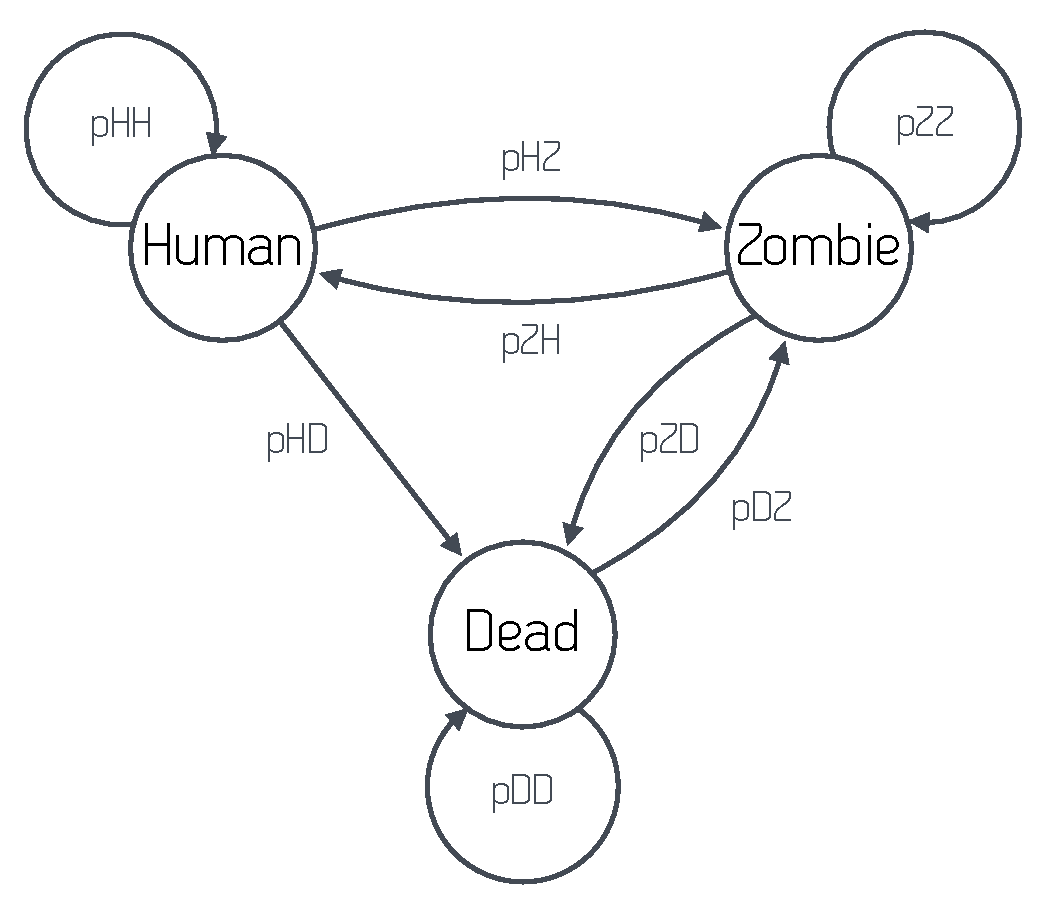
\includegraphics[width=90mm]{pics/MarkovZombie_title}
\end{figure}



\vfill

% Bottom of the page
{\large \today \\}

\end{center}
\end{titlepage} 

\linenumbers
\tableofcontents


%%%%%%%%%%%%%%%%%%%%%%%%%%%%%%%%%%%%%%%%%%%%%%%%%%%%%%%%%%%%%%%%%%%%%%
%%%%%%%%%%%%%%%%%%%%%%%%%%%%%%%%%%%%%%%%%%%%%%%%%%%%%%%%%%%%%%%%%%%%%%%
%%%%%%%%%%%%%%%%%%%%%%%%%%%%%%%%%%%%%%%%%%%%%%%%%%%%%%%%%%%%%%%%%%%%%%%
%%%%%%%%%%%%%%%%%%%%%%%%%%%%%%%%%%%%%%%%%%%%%%%%%%%%%%%%%%%%%%%%%%%%%%%
\chapter{Overview}

This document describes extensions and changes in \pml compared to version 0.6
 released in January 2015.


\section*{Major changes/extensions in version 0.7}
The following table summarises the major changes described in detail in following chapters. 
Please, note that this list is not exhaustive.

\captionsetup[longtable]{skip=1em}
\LTcapwidth=\textwidth
\begin{center}
%\renewcommand{\arraystretch}{1.1}%
\begin{longtable}{lll}
\hline
\hline
\pml element 				&  version $\le$ 0.7.2 			& version 0.8 \\
or modelling aspect 			& 							& \\
\hline
\hline
  \multicolumn{3}{c}{\textit{BIG TOPIC}}		\\
\hline
\hline
Section					& 							&	\\
\hline
\caption{Overview of major differences between versions 0.8 and 0.7.2.}
\label{figTable:overviewTable}
\vspace{-2em}
\end{longtable}
\end{center}



%%%%%%%%%%%%%%%%%%%%%%%%%%%%%%%%%%%%%%%%%%%%%%%%%%%%%%%%%%%%%%%%%%%
\input{input/Changes08}


%\appendix


%\paragraph{Covariate model}
%Covariate model is barely covered so far. See also \cite{Keizer:2011aa}. Missing are following features:\\
%For categorical covariates:\\
%-- categorical distribution of categorical covariates \\
%---- estimating categorical distribution from external data file -- TEST \\
%---- sampling from known categorical distribution -- TEST \\
%---- clusters of categorical covariates \\
%For continuous covariates:\\
%-- power-normal distribution for continuous covariates \\
%---- estimating parameters $\lambda$,$\mu$,$\sigma$ from external data file \\
%---- sampling from known power-normal distribution \\
%---- conditional distribution of continuous covariates - DONE \\
%---- selecting criteria for continuous covariates \\
%---- dependent distribution of continuous covariates \\
%---- correlated continuous covariates \\
%For both types: \\
%-- selection/exclusion criteria missing \\


\bibliographystyle{plain}
\bibliography{pharmml-specification}
\end{document}

